\documentclass{article}
\usepackage[utf8]{inputenc}
\usepackage[spanish]{babel}
\usepackage{listings}
\usepackage{graphicx}
\graphicspath{ {images/} }
\usepackage{cite}
\usepackage{subfig}
\usepackage{float}

\begin{document}

\begin{titlepage}
    \begin{center}
        \vspace*{1cm}
            
        \Huge
        \textbf{Parcial 1 - Calistenia}
            
        \vspace{0.5cm}
        \LARGE
        instrucciones
            
        \vspace{1.5cm}
            
        \textbf{Jesus David Tovar Serrano}
            
        \vfill
            
        \vspace{0.8cm}
            
        \Large
        Despartamento de Ingeniería Electrónica y Telecomunicaciones\\
        Universidad de Antioquia\\
        Medellín\\
        Marzo de 2021
            
    \end{center}
\end{titlepage}

\tableofcontents
\newpage
\section{Descripción del problema}\label{intro}
Este ejercicio consiste en describir cómo llevar unos objetos, en este caso dos tarjetas del mismo tamaño, de una posición inicial A una posición final B, para luego Poner a prueba la solución generada. Para esto le daré el documento con la descripción propuesta a tres personas, sin darles más instrucciones que seguir rigurosamente la guía del documento. La persona deberá realizar el ejercicio de forma autónoma sin preguntar nada a quien creo la solución, pues la única herramienta deber ser el documento con las instrucciones.

\section{Guía de solución} \label{contenido}
Con el objetivo de crear una posible solución al problema he creado una serie de pasos a seguir para que cualquier persona logre llevar las tarjetas de su posición inicial a su posición final.

\begin{enumerate}
  \item Por favor siga las siguientes instrucciones de manera rigurosa:
  \begin{enumerate}
  
  \item Para realizar de manera adecuada los siguientes pasos, lo primero que debes hacer es buscar una hoja tamaña A4 o carta, dos tarjetas del mismo tamaño, cuyo peso sea aproximadamente el mismo, y además debes usar una mesa o escritorio con una superficie plana para apoyarte durante la realización de los pasos que siguen.
  
  \item Sobre la mesa o escritorio, coloca las dos tarjetas, una sobre la otra, de manera que sus bordes queden alineados, y luego coloca la hoja sobre ambas tarjetas tratando de distribuir de la manera más equitativa el espacio de esta que no está siendo ocupado por la región o superficie de las tarjetas, es decir trata de ubicar la hoja de manera centrada sobre las tarjetas. A partir del siguiente paso solo puedes realizar las acciones que se describirán con una sola mano durante todo el tiempo hasta finalizar todos los pasos. (use su mano de preferencia)
  
  \item Toma la hoja con una sola mano y colócala en otro lugar de la misma mesa distinto al de las tarjetas, de manera que la parte más larga de la hoja quede vertical respecto a tu posición.
  
  \item toma por el extremo uno de los dos lados más largos de la hoja, y debes juntarlo con el otro de manera que se alineen, luego marca el lugar donde se doblan haciendo presión con la mano, así sabremos la mitad de la hoja, luego aplana la hoja de nuevo.
  
  \item toma una de las dos tarjetas y ubícala de manera horizontal en ese punto que se marcó en el paso anterior (centro vertical de la hoja), tratando de distribuir el área superficial de la tarjeta de manera equitativa, tal como lo indica la figura (\ref{estado 1})
  
  \item coloca tu dedo pulgar y has presión sobre la tarjeta para evitar que se mueva, con el resto de los dedos pliega el borde de lado largo de la hoja que este más cercano al resto de dedos, luego realiza la misma acción con el borde opuesto al plegado, Asegúrate de plegar bien ambos bordes hacia la posición de la tarjeta de manera que la cubran. ver borde a plegar en la figura (\ref{estado 2})
  
  \item abre cada borde plegado hasta formar un Angulo recto con la superficie de la mesa, luego saca la tarjeta agarrando con dos o tres dedos por los dos lados más largos de la tarjeta y sin soltarla toma la otra tarjeta que esta sobre la mesa de igual manera, sin llegar a juntarlas, es importante que tengan una separación así sea mínima.
  
  \item con las tarjetas en tu mano y en posición vertical respecto a la mesa, presiona una sola de ellas levemente, mientras acomodas la otra de manera que el extremo corto superior de ambas se vaya juntado y las tarjetas vayan formando un triángulo abierto, tal cual como se hace cuando intentas construir un castillo de naipes, solo que esta vez lo harás con una mano y tus dedos deben quedar en la parte superior de las tarjetas para que puedas manejarlas más fácil.
  
  \item manteniendo esta posición en las tarjetas lleva las tarjetas a la hoja, y utiliza los pliegues que hiciste anteriormente como soporte para cada una de las tarjetas, de esta manera no se caerán al soltarlas, coloca las tarjetas de manera de su borde corto inferior coincida con la línea del pliegue y con tus dedos alinea los bordes superiores y mantén las tarjetas por 5 segundos en la posición de triangulo abierto, hasta que estés seguro de que si las sueltas se mantendrán en esa posición. el estado final debe ser como en la figura (\ref{estado 3}), siendo los bordes donde estan las etiquetas t1 y T2, los que fueron a abiertos a 90 grados.
  

  
\end{enumerate}
\end{enumerate}

\section{Estados referenciados} \label{imagenes}

\begin{figure}[H]
 \centering
  \subfloat[Estado 1]{
   \label{estado 1}
    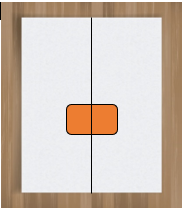
\includegraphics[width=0.3\textwidth]{1.png}}
  \subfloat[Estado 2]{
   \label{estado 2}
    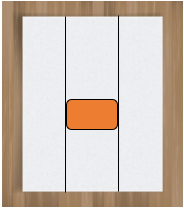
\includegraphics[width=0.3\textwidth]{2.png}}
  \subfloat[Estado 3]{
   \label{estado 3}
    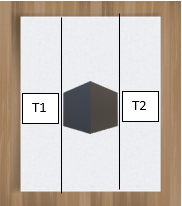
\includegraphics[width=0.3\textwidth]{3.png}}
 \caption{Estados}
 \label{f:estados}
\end{figure}

En la figura (\ref{estado 3}) T1 y T2 representan las dos tarjetas, además las secciones de pael donde estan escritas ambas etiquetas debven estar plegadas.


\section{Documentación de las pruebas realizadas con 3 personas}
En el siguiente link encontrara un video donde se registro el intento de 3 personas por resolver el problema:

youtu.be/kqlohikfwye

\end{document}
